\chapter{软件需求} % Introduction chapter suppressed from the table of contents
客户:公司准备推行软件需求与研发分离。\\
我:为什么要分开?\\
客户:公司希望可以提高需求的独立性,也希望需求可以与研发相互制衡。以前需求是研发团队的一部分,很多时候就会倾向于从研发团队的角度来看需求。分开后可以更加独立,更多地从客户的视角看需求。\\
我们严格要求做需求评审,可否用评审结果来评判需求的质量?\\
我:我常常会问团队,需求评审找出的缺陷是越多越好,还是越少越好?如果有人说是越少越好,我就会继续问是否0缺陷就是质量最好,所以我们难以单纯地用评审发现的缺陷数去衡量需求的质量。\\
让我先分享一下是如何来衡量过程质量。例如如何衡量系统测试的质量。看产品交付后有多少缺陷遗漏。如果没有任何遗漏的缺陷,那就表示系统测试做得很到位。如果往前倒退一步,可以从系统测试或验收测试发现的缺陷数来评判需求、设计或者编码的质量,如测试出的缺陷多就表示质量不好。但测试工程师无法判断那些系统测试的缺陷是因为代码还是需求引起的,所以如果要判断需求的质量,就必须在团队迭代回顾时,让所有成员(包括需求、设计、编码、项目经理等)一起分析缺陷源自哪里。所以过程的质量必须要从它的下游结果来判断。\\
我:你们把需求与开发分家以后有没有遇到什么问题?\\
客户:遇到问题可不少,例如研发团队会说,你需求写得太简单了,没写清楚,无法开发。而需求人员却说,你要写到多细才可以开发,你可以给我一个标准吗?甚至有些较极端的研发人员,明知需求有问题,但是还是按需求的描述做开发。\\
我:你记得我们解读软件工程时,说需求与开发是不断优化、完善的循环过程。需求不可能一次性写好,而是先依据客户提出的一些初步的概念,内部与开发讨论,然后再与客户交流,慢慢细化的。但如果把需求与开发切开,就切断了这个交流的过程。

软件开发一直困惑要怎么写好需求,但一直都没有找到能写出完美的需求文档、开发出完美的软件产品的秘方。有些团队为了写好需求文档,花了很多精力,但后面开发出来的产品还是问题多多,
甚至失败。所以在2001年时,17位敏捷大师针对当时瀑布式开发侧重文档的弊端,提倡敏捷开发,希望更有效地开发出客户满意的软件产品,而不是把时间浪费在前期文档上。敏捷开发模式也能更好地应对当时需求经常变化,导致后面项目延误和质量不好的问题。所以如果硬要将需求、研发分离,就是回到之前那种瀑布式开发的思路:花大量的精力希望写一个完美的需求文档。(敏捷开发的思路:软件开发的蓝图不是设计文档,也不是需求文档,而是代码本身。只有一个跑得动的代码,才是一个可交付、持久的东西。)

50年代针对英国煤矿生产问题的研究(详见附件)证明,要提升生产率不能单靠科学化的过程管理来实现,还必须有团队内部的相互合作。采煤这类传统低科技行业尚且需要团队合作,软件开发就更依赖于知识工作者的团队合作了。

客户:我们公司领导希望利用标准化的流程跟一些相关的度量指标去控制整个过程。我就是负责制定这些指标的。但有个问题,比如我们觉得研发做出来的产品应该得到客户的认同、让客户满意。所以客户满意度应该是个很重要的指标项。但研发组长就拒绝了这个指标,他说现在需求不是我们负责,我们只是做研发,为什么最终那个产品的满意度要由我们研发负责,因为我们控制不了需求的质量。如果我们要需求人员或者产品经理对最终的客户满意度负责,体现在KPI指标,他们也会说,研发不是我们管,我们只做需求,开发做出来的产品客户不满意,为什么让我们买单?其实两边都有道理。如果我们希望只通过一些指标,比如针对研发的指标,反而会对总体的效果有负面影响,比如客户满意度。但是大家也知道,如果客户对一个产品不满意,那开发肯定有问题。所以只度量某些过程没有意义,就好比如果评审或者测试的缺陷数越高,奖励越多,聪明的团队可以很轻松地变成百万富翁。人很聪明,针对指标,他们都会有方式达到要求。\\
客户:你说得很对,我们那些团队就很懂怎么朝那个指标作假。\\
我:所以要有合理的度量,尤其是和奖励挂钩的度量就必须是客观、项目间可比和全面。例如最终盈利多少比较客观,或客户满意度指标也可以很好地激励团队之间相互合作的积极性,对公司、对团队都有好处。但是如果只是用个别过程的指标去衡量,反而可能影响团队行为。\\
客户:公司觉得今年改革之前做新产品开发项目的立项太宽松,缺乏有效的管理和监督,这导致很多新的研发项目都是没有回报或者失败,浪费了很多资源。所以现在用新方式,所有立项的研发项目,都应该由中央委员会审批才能立项和开始做,我觉得这个倒是挺好的。\\
我:你觉得好吗?\\
你听过苹果公司的故事吗?苹果公司本身就是由两人创办:
一位是我们都认识的乔布斯、另外一位是沃兹(Steve
Wozniak),他本来是惠普的工程师,在75~76年间研发出了苹果电脑(Apple
1),本来希望获得惠普高层的支持,就申请内部立项,但多次都被拒绝。乔布斯看到这个产品后,觉得很有市场潜力,就跟沃兹跑市场,最终获得Byte
Shop 老板 Paul Terrell的首张订单,购买了200套苹果电脑(Apple
1)。当时Apple 1 都由沃兹手工焊接而成。创新产品都必须具备以下重要元素:

\begin{enumerate}
\tightlist
\item
  了解市场需求的人员,乔布斯就是这个角色。
\item
  研发工程师沃兹。
\end{enumerate}

两者相互合作才把苹果产品做成。如果把需求跟研发切开,估计苹果的传奇故事永远都不会诞生。正是两人的团队合作,一起去满足个人电脑需求的市场才会成功。从这个例子可以知道,要创新就不能用传统的工厂化流程,靠一些指标去管理。所以若单依赖一些质量指标去管理需求和研发过程,是不利于团队与公司的健康发展。

惠普公司很优秀,内部肯定不缺资深专家,评判的指标也应该很完善,为什么沃兹的内部申请立项,多次都被拒绝?惠普一直都是专注于做度量和测量仪器,但个人电脑是全新的概念,所以单靠现有专家的指标是无法鼓励项目创新。发明全新的东西必须是需求配合技术开发工程师,再有客户的接触跟确认,才可以成功实现。

客户:有道理,我们现在在新方式下几乎都没有什么创新了,都是按以前的方式做。\\
我:但这正是软件开发公司最致命的问题,没有创新,后面就会被竞争对手超越。\\

\hypertarget{ux9644ux4ef6}{%
\section{附件}\label{ux9644ux4ef6}}

\hypertarget{ux82f1ux56fdux7164ux77ffux751fux4ea7ux95eeux9898ux7684ux7814ux7a76}{%
\subsection{英国煤矿生产问题的研究}\label{ux82f1ux56fdux7164ux77ffux751fux4ea7ux95eeux9898ux7684ux7814ux7a76}}

在机械化之前,英国采煤是以小组作坊式工作,通常是两人一组,再加上一位做清理的助手。小组会直接跟矿场合作,专门负责某一块煤矿,小组以互补的形式做各种工作,自己管自己,独立性很高。因为采矿工作非常危险,所以选择伙伴很重要,都希望有稳定的伙伴关系,不会轻易换人。当某工人受伤或者去世,他的伙伴都会尽力帮助他的家人。这种小组作坊式工作方式后来被机械化生产线模式取代,但机械化生产却引起很多新问题。

先了解一下长壁(Longwall)开采法是怎么利用机械化大规模开采煤矿。

煤是古代的植物经过很多年的碳化累计下来的产物,英国的煤层一般不深,最多可能一米左右,上面覆盖着泥土。用长壁机械化采煤方式就可以大面积采煤。我们看看它是怎么操作的。

%\url{文件:langwall-修改56.2.jpg}

\includegraphics[width=6cm]{langwall-修改562.jpg}

(上图A部分是煤矿俯视图,B部分是俯视图中右到左横虚线的切面图,都能看到是左、中、右3条隧道)

共180米宽的长壁是为了大面积采煤,(看上图)为了通风和运输,会有3条隧道,之间距离90米,中间隧道是比较高,大概有3米(9英尺),左右隧道比较矮,大概2米(6英尺)高。这些隧道都是固定,让人或者那些机械也可以在中间运输。看上面平面图,粉红色是已经采完煤的泥土。从下面的切面线可以看到中间的和两边两个隧道。每个采煤的煤层,只有1米高。也可以看见红色的柱子,柱子是用来顶住上面的泥土,防止泥土在煤挖空以后塌下来。

%\url{文件:langwall2-修改5.2.jpg}

\includegraphics[width=6cm]{langwall2-修改52.jpg}

(图2 说明:与图1 类似,A部分是俯视图(平面图),B部分是横的切面图)

可以从上面那平面图理解整个长壁(Longwall)如何操作。右面就是已经采完煤的那些泥土,我们用粉红色标注,叫GOB。右面有两条垂直的过道,都是1米宽。前面两米宽的那条过道,是之前已开采完的,它左面会有一条传输带运作的通道,右面是一条只有1米高的通道,以便采煤工人爬过去工作。你可以想象环境多么恶劣。左面那个通道就是一条新建的通道,同样它左面是传送带,右面是矿工爬行通道。每一次采完右面的煤以后,有工人会把那些柱子拆掉,放到新的通道里面,然后再依据这条通道挖左面的煤,一直往左边伸。你可以想象在第一个图的左、右面90米宽的长壁,就是一个连续往上升的一条线,矿工按分配的工种和轮班去挖煤。为了配合这种机械化挖煤方式,工人就不能再用以前的作坊式小组工作。工业工程师设计了7个工种,请参照下面的轮班表。每循环会包括3个轮班:

\begin{itemize}
\tightlist
\item
  第1个轮班主要是做转动和切割和清理,比如让那些切割的煤有空位落下来,让后面那些采煤工人容易可以采到煤。通常第一个轮班都是下午班或者晚班。
\item
  第2个轮班就是巩固隧道和安装传输带,通常是下午班或者晚班,这2个班总共就会大概有20个工人。细分到不同的工种,比如有2位只钻洞、2位只切割、8位专门管理通风隧道的巩固工作,分工很细。
\item
  第3个轮班主要有20位采煤工人操作。第3个轮班只有早上班和下午班,所以他们需要依赖前期技术人员做好准备工作,然后自己按大概9米的范围去采煤。收入是按采煤量计算,比如20个采煤人每人负责9米,加起来刚好等于整个长壁的180米。
\end{itemize}

分工设计很科学,如果都按正常操作,每次循环可以采到200吨煤。

%\url{文件:长壁1.1.jpg}

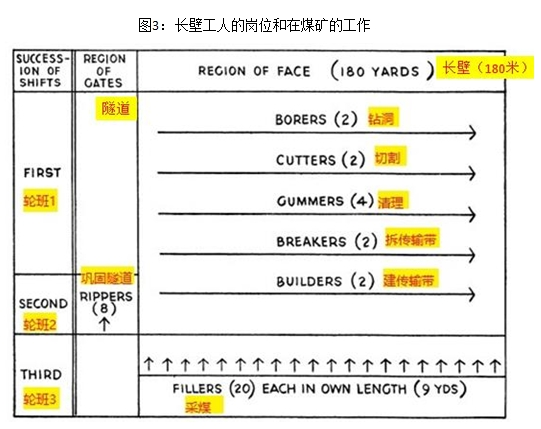
\includegraphics[width=6cm]{长壁11.jpg}

但是你估计,这种机械化的大规模连续采煤操作会有什么问题?生产力效果怎么样?

以上的工作关系很密切,例如:

\begin{itemize}
\tightlist
\item
  如果洞钻得不够深,采煤工便采不到煤。
\item
  如果切割没做好会导致采煤工可采空间不足,影响产量。
\item
  如传输带没有安装好,不成直线就导致后面的传输停顿,采煤工无法操作。
\end{itemize}

各种状况都可能发生,加上煤矿是天然的,本身就有很多变数:例如地层有断层,或者地下天然气等。各种人为因素或天然因素都影响采煤工能否正常采煤。加上采煤的工作环境很恶劣,导致旷工问题很严重。例如某采煤工因前面2个轮班工作没做好,导致煤太硬,采不了,就需要用机器、工具去采,很辛苦,效果也不好,导致他工作2天就放一天假,然后也不补班。有些轮班因为人手不够,剩下的采矿工人就需要在地下多做两三个小时,才可以把整个长壁做完。最后当有些轮班时,采矿人数确实太少了,其他人也撂担子,导致无法正常开工。\\
因为采用机械化大规模采煤的各种问题,有些矿场开始引入自主团队组织架构
取代原本的轮班分工(下面称为传统分工)

表1是两个不同的组织架构,技术都一样,也是在同一个环境。左面用原本长壁的方式设计工作分工,右面的加上自主团队负责制分工。左面矿工只需要做一项简单工作,比如采煤,与其他工人没有任何关系(在前面已详细举例说明)。右面就需要组员合作,协调应对采矿的各种特殊情况。\\
从这个例子看到同样一个采煤技术,可以有不同的组织架构支撑,效果完全不一样。所以团队组织架构必须与技术部分相配合,不能单独设计工人工作。

%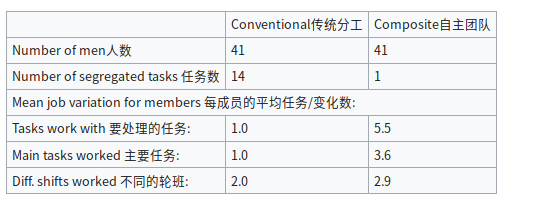
\includegraphics[width=6cm]{Screenshotfrom2023-11-0303-25-17.png}

\begin{tabular}{|c|c|c|}
\hline
\:&Conventional传统分工&Composite自主团队\\
\hline
Number of men人数&41&41\\
\hline
Number of segregated tasks 任务数&14&1 \\
\hline
\multirow{3}{*}{Mean job variation for members 每成员的平均任务/变化数: }\\
\hline
Tasks work with 要处理的任务:&1.0&5.5\\
\hline
Main tasks worked 主要任务:&1.0&3.6\\
\hline
Diff. shifts worked 不同的轮班:&2.0&2.9\\
\hline
\end{tabular}


从下面表2可以看到右面的组织架构更灵活,生产率比传统的单一工作设计高。右面的自主团队架构更能适应变化万千的采矿、采煤环境。采煤的步骤安排,也必须按照按环境的不同来应对。但如果是左面的硬性单一分工安排,缺乏这种灵活性(除非是专业性强的技术工种,必须把工作细分,每个人做某一件事)。但在采煤机械化、批量生产这种技术没有这个限制,所以采煤工人经过一些学习可以兼任其他工作。

%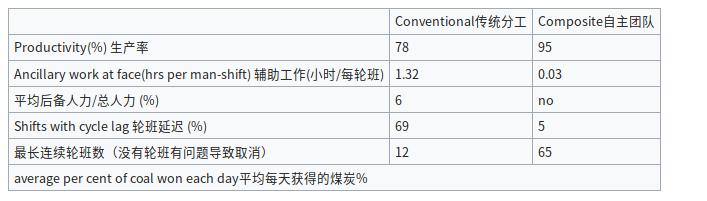
\includegraphics[width=6cm]{Screenshotfrom2023-11-0303-25-45.png}

\begin{tabular}{|c|c|c|}
\hline
\:&Conventional传统分工&Composite自主团队\\
\hline
Productivity(\%) 生产率&78&95\\
\hline
Ancillary work at face(hrs per man-shift) 辅助工作(小时/每轮班)&1.32&0.03 \\
\hline
平均后备人力/总人力 (\%)&6&no\\
\hline
Shifts with cycle lag 轮班延迟 (\%)&69&5\\
\hline
最长连续轮班数(没有轮班有问题导致取消)&12&65\\
\hline
\multirow{3}{*}{average per cent of coal won each day平均每天获得的煤炭\%}\\
\hline
\end{tabular}


团队组织架构除了让工人更好做好采矿工作以外,也可以更好满足工人的个人心理需要,包括互相支持,有团队合作的概念。但是如果按左面传统的工业化分工,就缺乏合作。导致很多采煤工只能单打独斗,孤立无援,导致心理压力很大。这个也可以从表3的缺勤率看得出来,会更容易无缘无故请假等,背后主因是分工设计导致工人心理压力太大,承受不了。团队互相协助的环境可以减轻这方面的压力。

%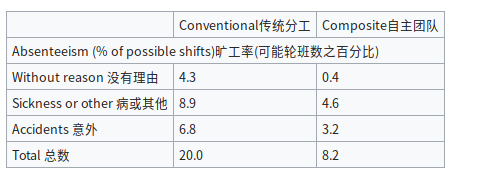
\includegraphics[width=6cm]{Screenshotfrom2023-11-0303-26-09.png}

\begin{tabular}{|c|c|c|}
\hline
\:&Conventional传统分工&Composite自主团队\\
\hline
\multirow{3}{*}{Absenteeism (\% of possible shifts)旷工率(可能轮班数之百分比) }\\
\hline
Without reason 没有理由&4.3&0.4 \\
\hline
Sickness or other 病或其他&8.9&4.6\\
\hline
Accidents 意外&6.8&3.2\\
\hline
Total 总数&20.0&8.2\\
\hline
\end{tabular}


